%======================================================================
%  Anexo C - Implementacion del modelo global en la herramienta CASE
%======================================================================

\section{Implementación del modelo global en la herramienta CASE}
\label{anx:case}


El modelo se implementó en Oracle SQL Developer Data Modeler, la
herramienta CASE del curso. En ella se equivalen los nombres de la
siguiente manera: lo que la herramienta llama \textit{Logical Model}
corresponde al modelo conceptual de este capítulo (entidades, atributos
y relaciones), y lo que llama \textit{Relational Model} corresponde al
modelo lógico del capítulo 4 (tablas, claves primarias y claves
foráneas).

En la herramienta se construyeron tres diseños: el prediseño
(figura~\ref{fig:erintegradoglobal}), la vista U7
(figura~\ref{fig:vistaU7}) y el modelo ajustado
(figuras~\ref{fig:erfinalA} y~\ref{fig:erfinalB}). Como las vistas U2,
U3, U4, U5, U6 y U8 son subconjuntos del prediseño
(sección~\ref{sec:integracion}), se construyeron como subvistas
(\textit{SubViews}) del diseño del prediseño; la vista U7 tiene su propio
diseño porque incluye la relación CLIENTE--\textit{envía}--ENVIO, que no
pasó al modelo integrado.

La herramienta representa el modelo en notación Barker. La
tabla~\ref{tab:barker} muestra su equivalencia con la notación de Chen
usada en el capítulo 3.

{\singlespacing
\begin{longtable}{L{4.0cm} L{5.4cm} L{5.0cm}}
\caption{Equivalencia entre la notación Barker de Data Modeler y la notación de Chen.}
\label{tab:barker}\\
\toprule
\textbf{Elemento} & \textbf{Barker (Data Modeler)} & \textbf{Chen (capítulo 3)} \\
\midrule
\endfirsthead
\toprule
\textbf{Elemento} & \textbf{Barker (Data Modeler)} & \textbf{Chen (capítulo 3)} \\
\midrule
\endhead
\bottomrule
\endfoot
Entidad & Rectángulo de esquinas redondeadas con el nombre y la lista de atributos & Rectángulo con el nombre \\
Atributo obligatorio u opcional & Marcado con \texttt{*} (obligatorio) u \texttt{o} (opcional) & No se dibuja; está en las tablas~\ref{tab:entidades} y~\ref{tab:atributosajustados} \\
Identificador & \texttt{P} (identificador principal) y \texttt{U} (valor único) & Primer atributo de la tabla de entidades \\
Relación & Línea entre las dos entidades, sin nombre visible & Rombo con el nombre de la relación \\
Cardinalidad máxima N & Pata de gallo en el extremo de la entidad & N en la pareja (mín, máx) \\
Participación & Mitad de línea continua: obligatoria; discontinua: opcional & Mínimo 1 u 0 en la pareja (mín, máx) \\
Relación identificadora & Barra transversal en el extremo de la entidad dependiente & No aplica en este modelo \\
Relación N:M con atributos & Entidad intermedia con dos relaciones identificadoras & Rombo con elipses de atributos \\
\end{longtable}
\par}

Al comparar los diagramas de la herramienta con los de Chen se deben
tener en cuenta cuatro diferencias, que se deben a la notación y no a
cambios en el modelo:

\begin{enumerate}[label=\arabic*.,leftmargin=1.2cm]
  \item \textbf{Relaciones N:M.} Las relaciones \textit{se asigna},
        \textit{asiste} y \textit{exige} aparecen como las entidades
        intermedias ENVIO\_DESPACHO, ASISTENCIA y DOCUMENTO\_EXIGIDO. Por
        eso el prediseño tiene 23 entidades en la herramienta (21 en
        Chen) y el modelo ajustado tiene 30 (28 en Chen).
  \item \textbf{Mínimo del lado ``uno''.} Una clave foránea no puede
        exigir que un registro padre tenga al menos un hijo, así que la
        herramienta dibuja siempre como opcional el extremo del lado
        ``uno''. Las
        relaciones \textit{tiene}, \textit{pacta}, \textit{contiene},
        \textit{registra}, \textit{incluye}, \textit{cubre} y
        \textit{dirigido} tienen mínimo 1 en ese lado en el modelo de
        Chen; esa regla se controlará en el diseño físico.
  \item \textbf{Especialización.} MENSAJERO aparece como una relación 1:1
        identificadora con EMPLEADO, porque su identificador es el mismo
        del empleado. Representa la misma especialización parcial de la
        figura~\ref{fig:erfinalB}.
  \item \textbf{Claves foráneas.} El modelo lógico de la herramienta no
        muestra las columnas de clave foránea; estas aparecen en el modelo
        relacional del capítulo 4.
\end{enumerate}

Cada diagrama de la herramienta se verificó contra su diagrama de Chen,
relación por relación. Los resultados de la tabla~\ref{tab:verificacion}
coinciden en todos los casos en entidades, relaciones, cardinalidad
máxima y participación del lado ``muchos''.

{\singlespacing
\begin{table}[H]
\centering
\caption{Verificación de los diagramas de Data Modeler.}
\label{tab:verificacion}
\small
\begin{tabular}{L{5.6cm} L{2.8cm} c c c}
\toprule
\textbf{Diagrama} & \textbf{Diseño} & \textbf{Entidades} & \textbf{Relaciones} & \textbf{Figura} \\
\midrule
Vista U2 -- Personal del centro & Prediseño & 13 & 17 & \ref{fig:dmU2} \\
Vista U3 -- Mesa de servicio & Prediseño & 11 & 14 & \ref{fig:dmU3} \\
Vista U4 -- Mensajero & Prediseño & 10 & 11 & \ref{fig:vistaU4} (cap. 3) \\
Vista U5 -- Flota & Prediseño & 5 & 5 & \ref{fig:dmU5} \\
Vista U6 -- Comercial & Prediseño & 6 & 6 & \ref{fig:dmU6} \\
Vista U7 -- Facturación y cartera & Vista U7 & 6 & 7 & \ref{fig:dmU7} \\
Vista U8 -- Talento humano & Prediseño & 4 & 3 & \ref{fig:dmU8} \\
Modelo ajustado & Ajustado & 30 & 42 & \ref{fig:dmajustado} \\
\bottomrule
\end{tabular}
\end{table}
\par}

\begin{landscape}
{\singlespacing
\begin{figure}[p]
\centering
\adjustbox{max width=22.5cm, max totalheight=14.6cm}{%%
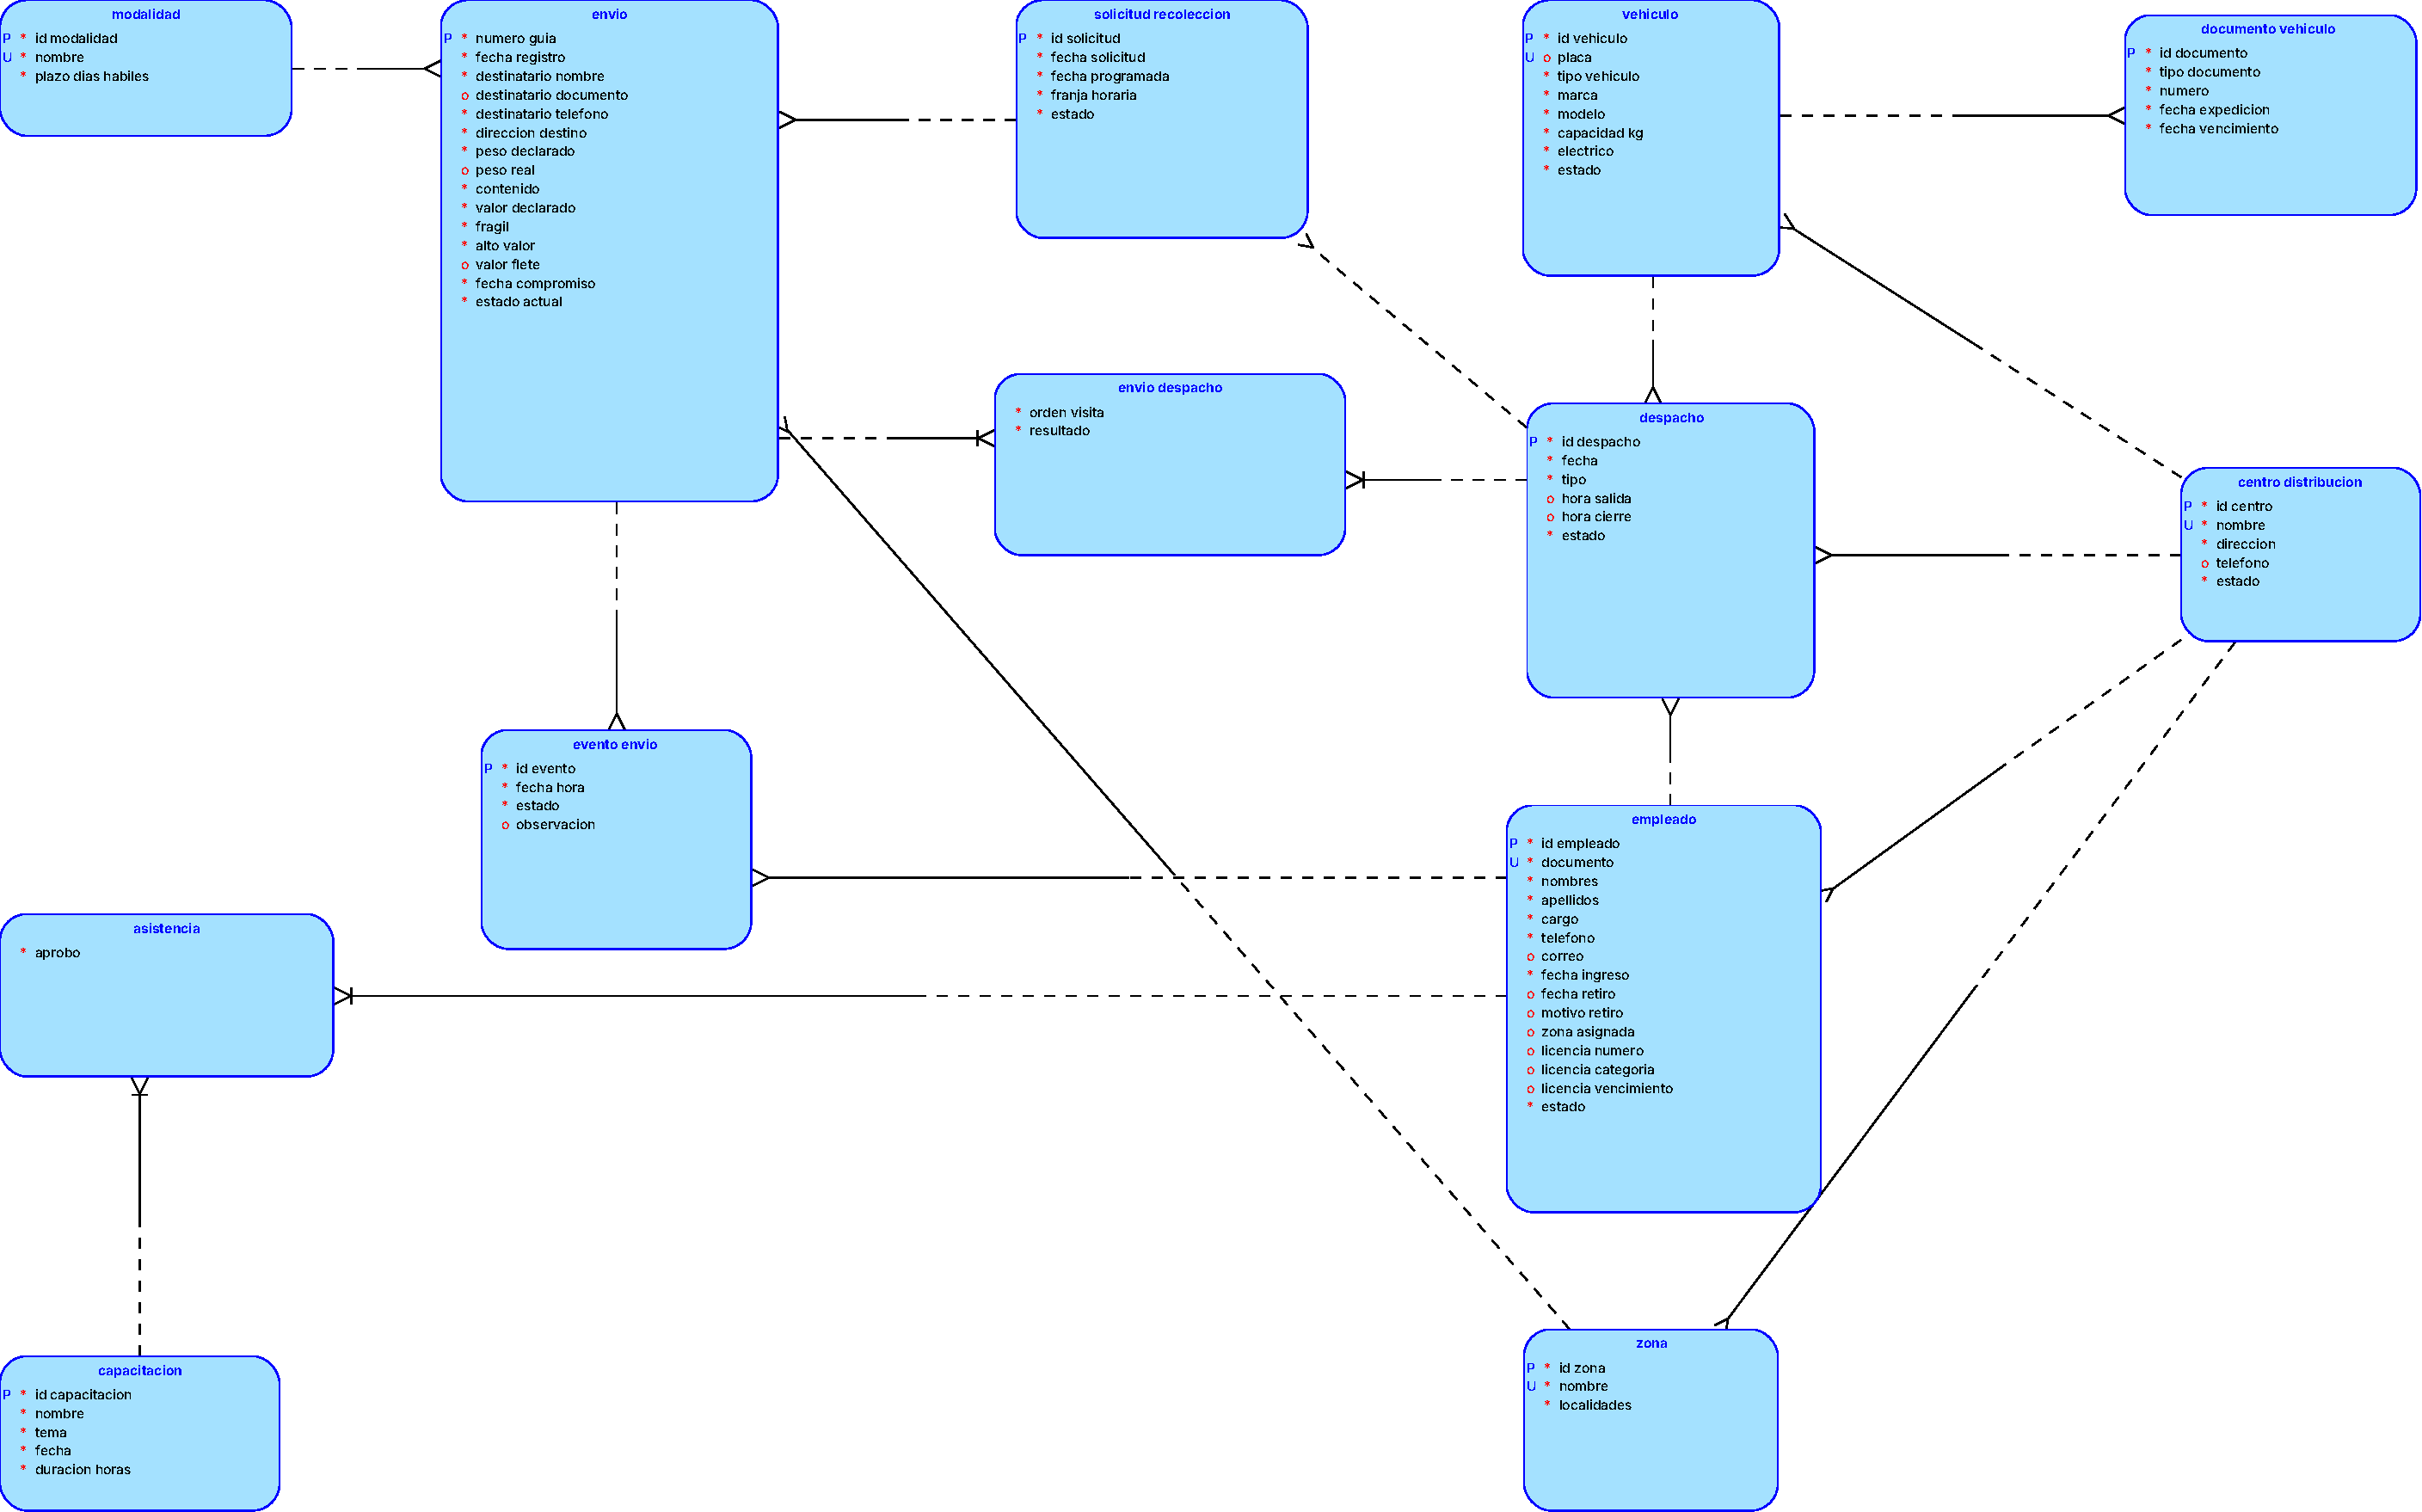
\includegraphics{figuras/datamodeler/dm_U2.pdf}
}
\caption{Vista U2 en Data Modeler (subvista del prediseño).}
\label{fig:dmU2}
\end{figure}
\par}
\end{landscape}

\begin{landscape}
{\singlespacing
\begin{figure}[p]
\centering
\adjustbox{max width=22.5cm, max totalheight=14.6cm}{%%
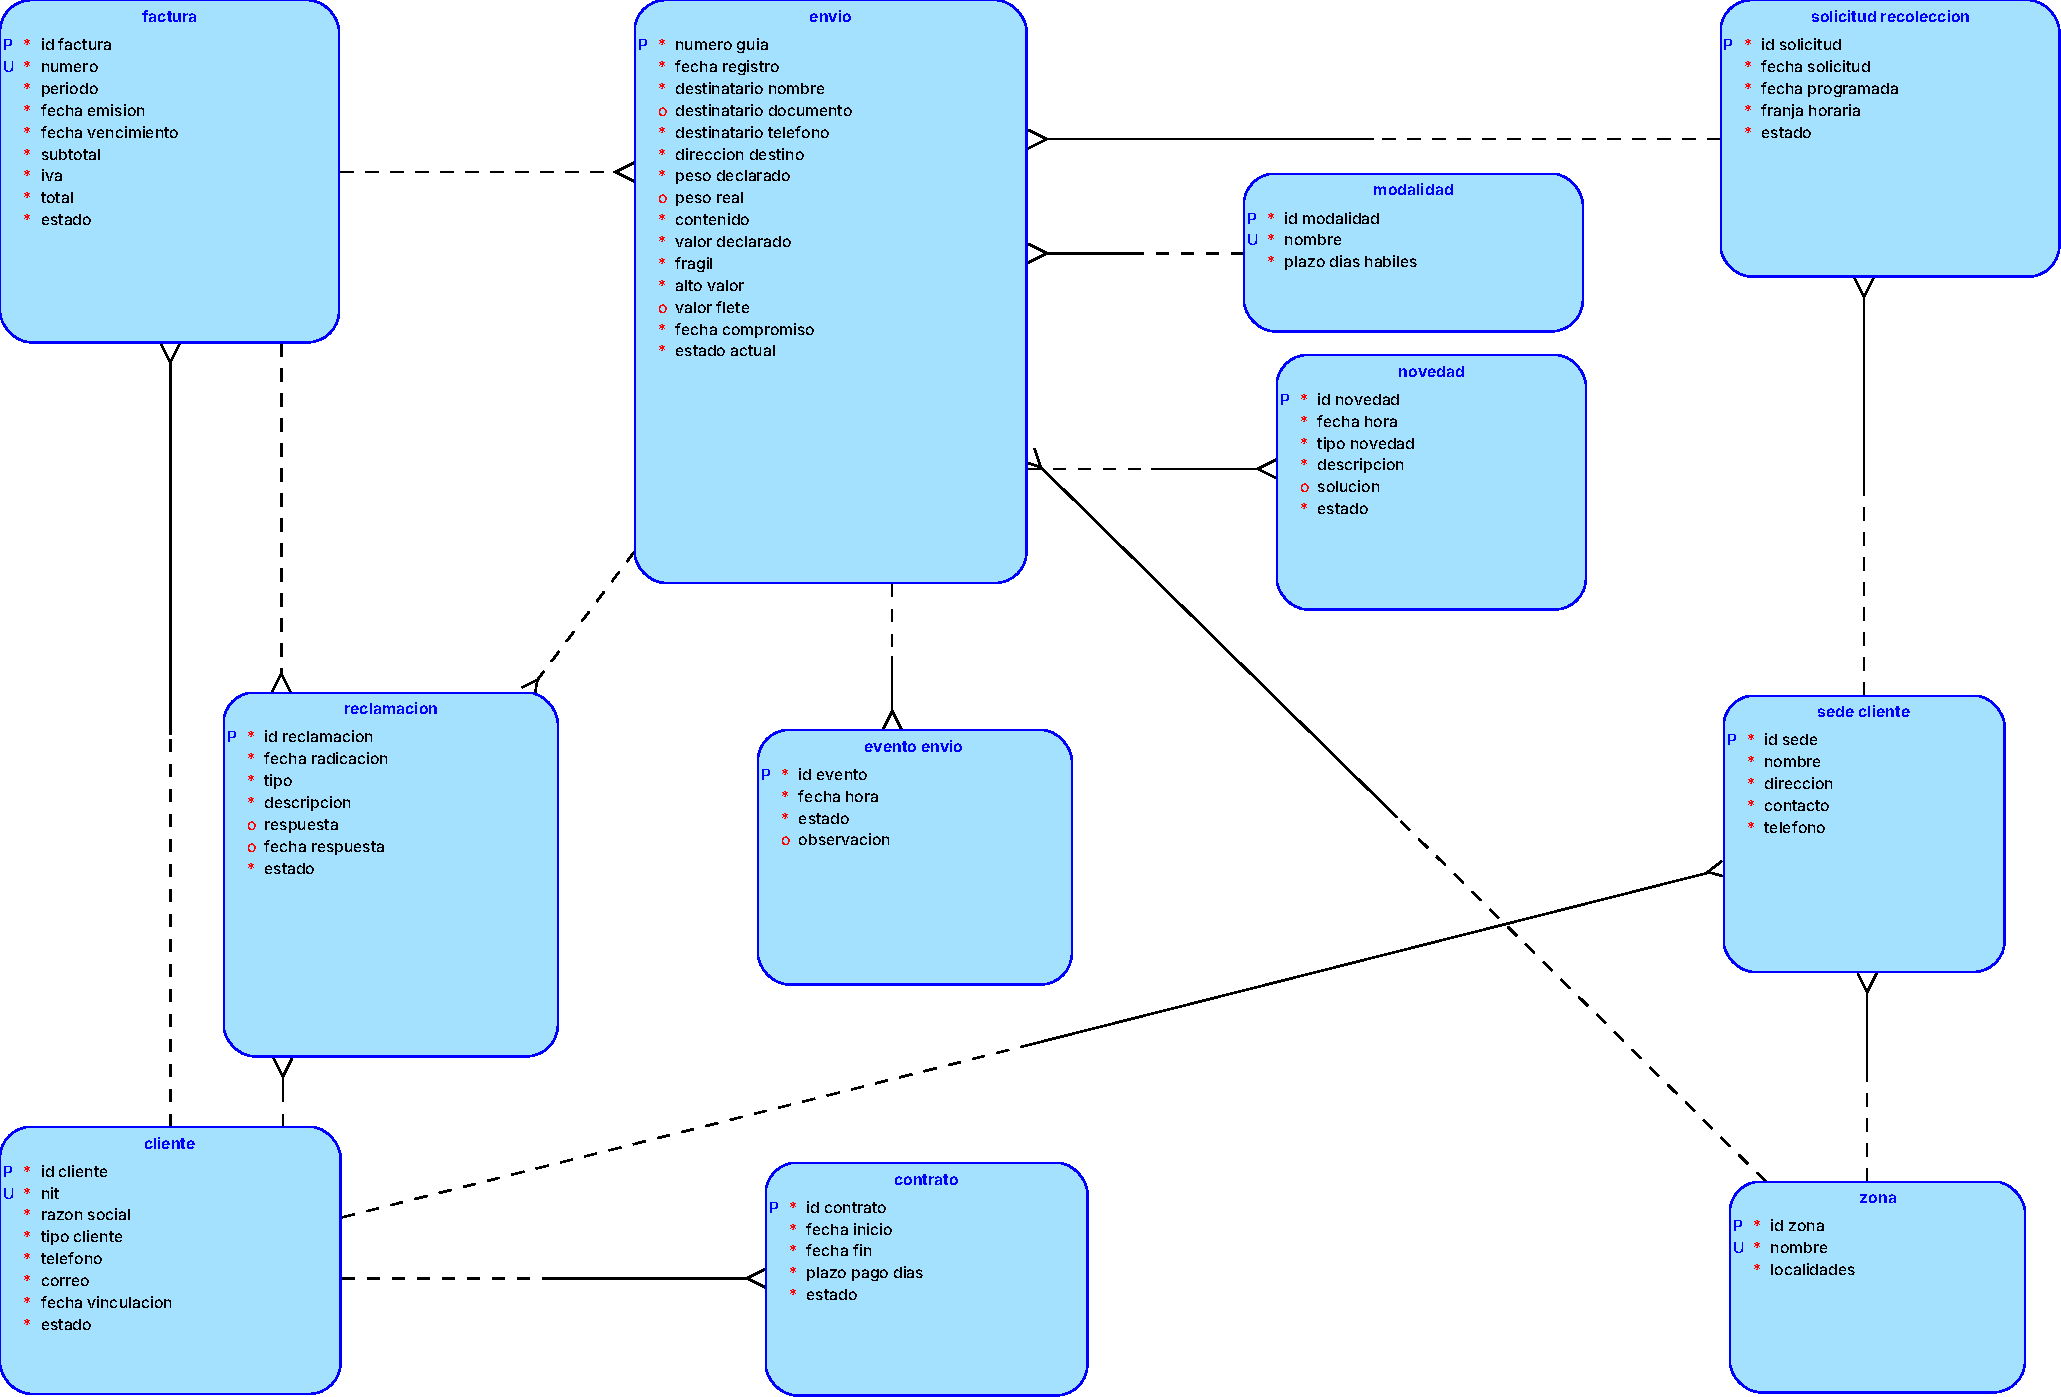
\includegraphics{figuras/datamodeler/dm_U3.pdf}
}
\caption{Vista U3 en Data Modeler (subvista del prediseño).}
\label{fig:dmU3}
\end{figure}
\par}
\end{landscape}

{\singlespacing
\begin{figure}[!htb]
\centering
\adjustbox{max width=\linewidth}{%%
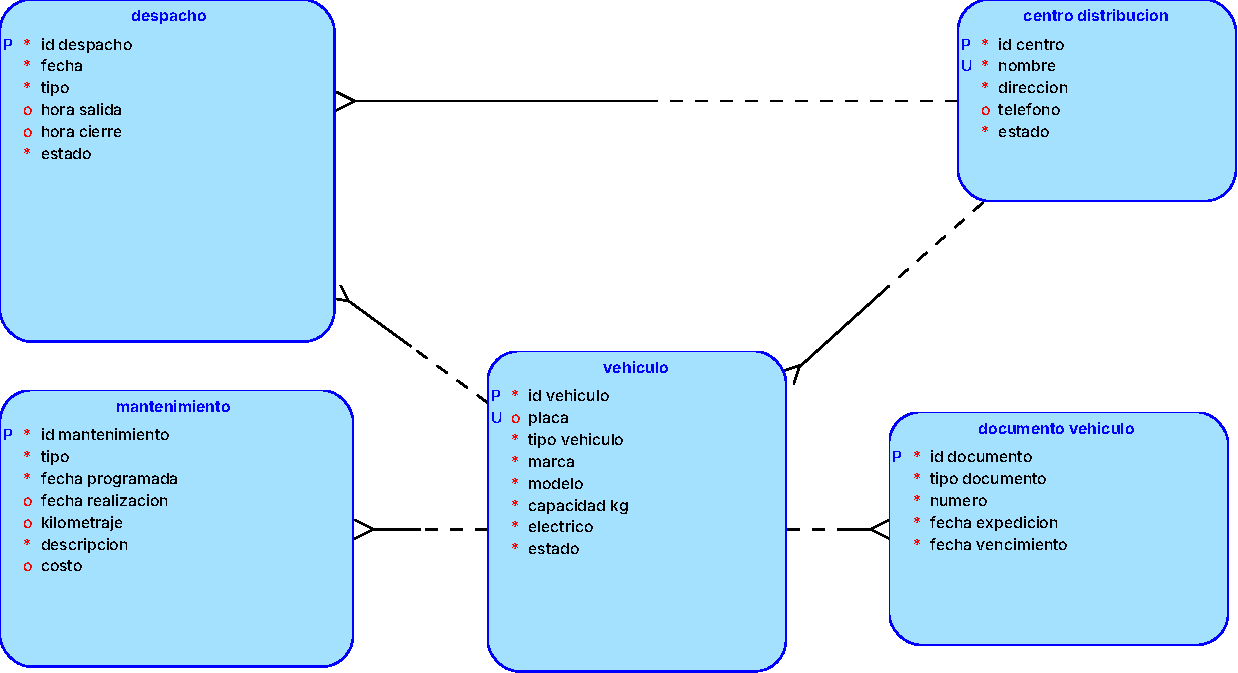
\includegraphics[height=0.62\textheight,width=\linewidth,keepaspectratio]{figuras/datamodeler/dm_U5.pdf}
}
\caption{Vista U5 en Data Modeler (subvista del prediseño).}
\label{fig:dmU5}
\end{figure}
\par}

{\singlespacing
\begin{figure}[!htb]
\centering
\adjustbox{max width=\linewidth}{%%
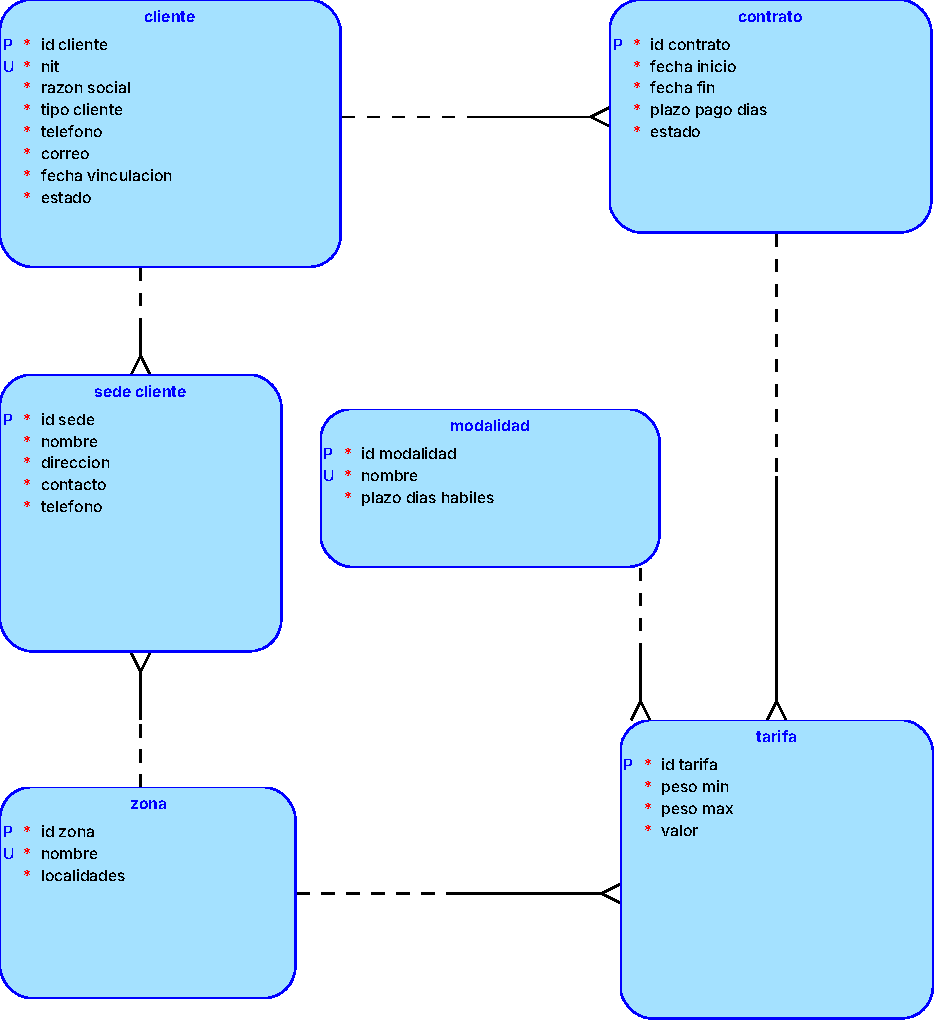
\includegraphics[height=0.62\textheight,width=\linewidth,keepaspectratio]{figuras/datamodeler/dm_U6.pdf}
}
\caption{Vista U6 en Data Modeler (subvista del prediseño).}
\label{fig:dmU6}
\end{figure}
\par}

{\singlespacing
\begin{figure}[!htb]
\centering
\adjustbox{max width=\linewidth}{%%
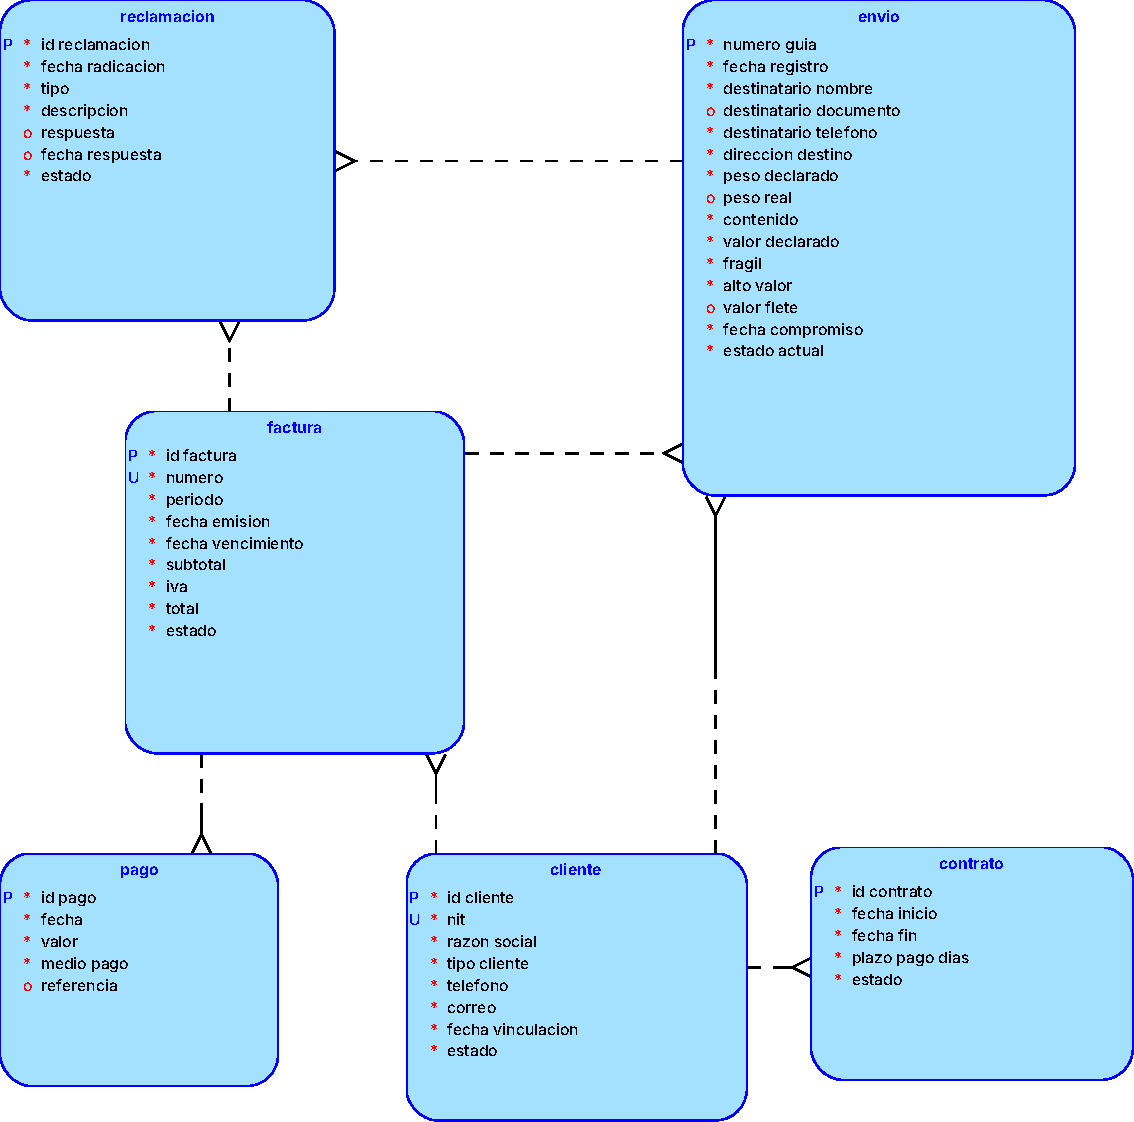
\includegraphics[height=0.62\textheight,width=\linewidth,keepaspectratio]{figuras/datamodeler/dm_U7.pdf}
}
\caption{Vista U7 en Data Modeler (diseño propio).}
\label{fig:dmU7}
\end{figure}
\par}

{\singlespacing
\begin{figure}[!htb]
\centering
\adjustbox{max width=\linewidth}{%%
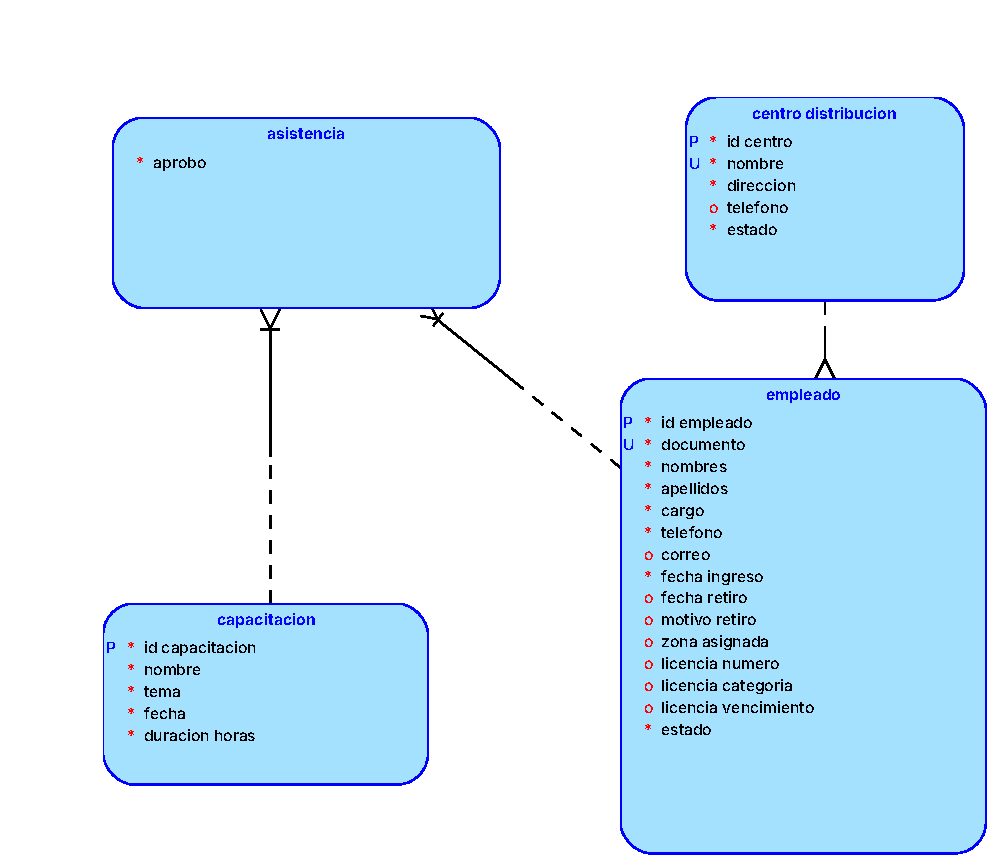
\includegraphics[height=0.62\textheight,width=\linewidth,keepaspectratio]{figuras/datamodeler/dm_U8.pdf}
}
\caption{Vista U8 en Data Modeler (subvista del prediseño).}
\label{fig:dmU8}
\end{figure}
\par}

\begin{landscape}
{\singlespacing
\begin{figure}[p]
\centering
\adjustbox{max width=22.5cm, max totalheight=14.6cm}{%%
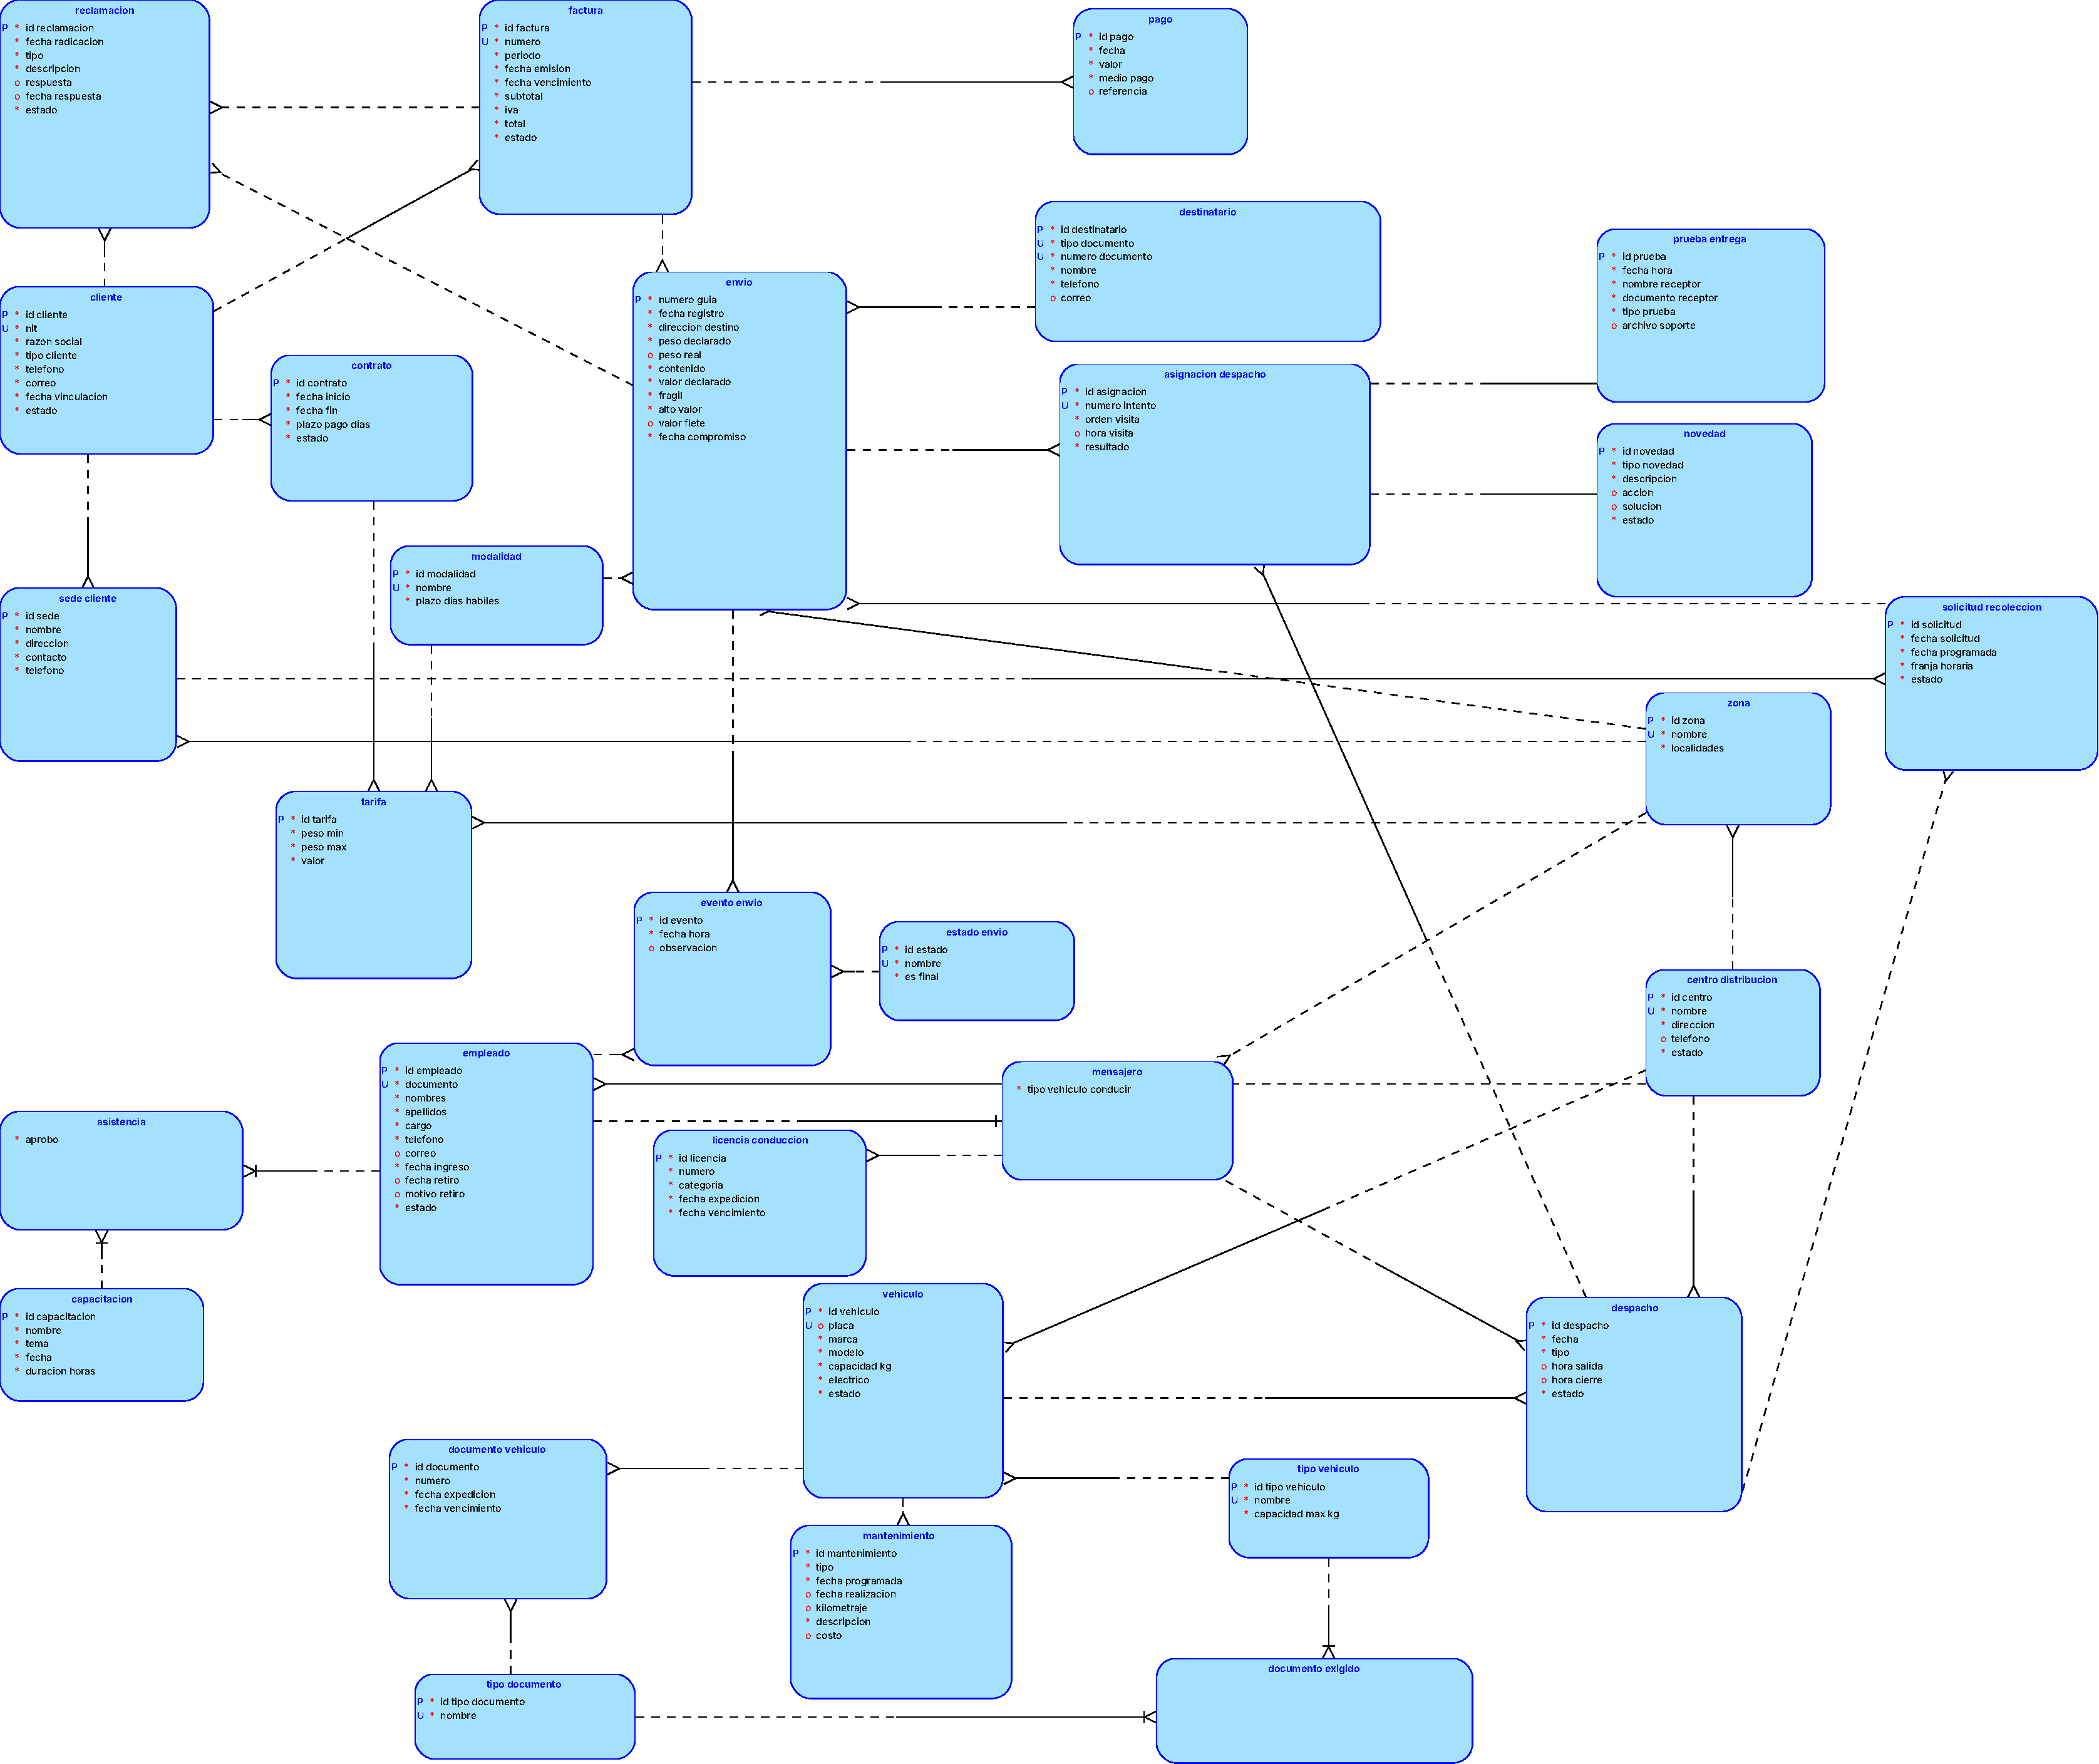
\includegraphics{figuras/datamodeler/dm_modelo_ajustado.pdf}
}
\caption{Modelo ajustado en Data Modeler (diseño completo, 30 entidades).}
\label{fig:dmajustado}
\end{figure}
\par}
\end{landscape}
